\documentclass{beamer}
\usepackage[latin1]{inputenc}
\usepackage{bm, array, graphicx, hyperref, amsmath, setspace, geometry, wrapfig}
\usetheme{Warsaw}
\title{Introduction to Nuclear Magnetic Resonance Spectroscopy}
\author{Dr Alexey Potapov}
\institute{University of Nottingham, School of Physics and Astronomy}
\date{Jule 13, 2017}

\setbeamertemplate{headline}{}
\setbeamertemplate{footline}{}
\setbeamertemplate{caption}{Fig.\insertcaptionnumber: \insertcaption \par}
\setbeamerfont{caption}{size=\scriptsize }
\setbeamercovered{invisible}
\setbeamercovered{%
	again covered={\opaqueness<1->{50}}}
%\newenvironment{slide}[1]
%{\begin{frame}[environment=slide]
%		\frametitle{\insertsection-#1}}
%	{\end{frame}}
\newcolumntype{C}[1]{>{\centering\arraybackslash}m{#1}}



\begin{document}
	
	\begin{frame}
		\titlepage
	\end{frame}
	
	\section{Introduction. Magnetic moment in magnetic field.}
	\subsection{Introduction to Magnetic Resonance}	
	\begin{frame}{\thesection.\thesubsection. \insertsubsection}

		
		\begin{itemize}
		\item Magnetic resonance (MR) is a phenomenon of resonant energy absorption by a system of nuclei (and electrons). 
		\item Nuclear magnetic resonance (NMR) results from the intrinsic magnetic moment of the
		nuclei of some atoms. Magnetic moments of electrons are exploited in electron spin resonance.
		\item Magnetic resonance (MR) generally involves placing a sample in a strong magnetic
		field (to generate polarisation at a fixed resonant frequency) and detecting signals
		produced following application of pulsed radio-frequency electromagnetic fields (RF
		pulses).
		\item MR is a very powerful method for studying the structure of materials: used in physics, chemistry, biology, medicine etc.

		\end{itemize}
	\end{frame}
	
	\subsection{Applications of NMR}
	\begin{frame}{\thesection.\thesubsection. \insertsubsection}
	 \begin{itemize}
	 	\item NMR spectroscopy is used for chemical analysis and for molecular structure determination	  	
	 \end{itemize}
		
		\begin{figure}[ht]
			\begin{minipage}[t]{0.45\linewidth}
				\centering
				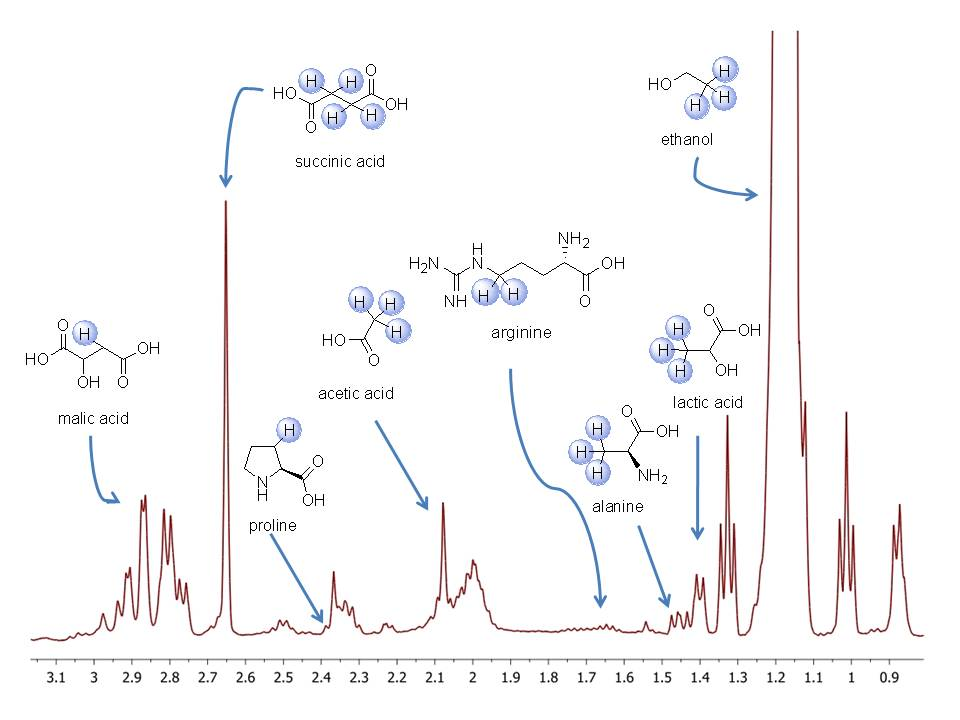
\includegraphics[width=\textwidth]{wine_spectrum.jpg}
				\caption{\textsuperscript{1}H NMR spectrum of a sample of Spanish wine (\url{http://www.unirioja.es/gsoe/NMR.htm})}
				\label{fig1}
			\end{minipage}
			\hspace{0.3cm}
			\begin{minipage}[t]{0.45\linewidth}
				\centering
				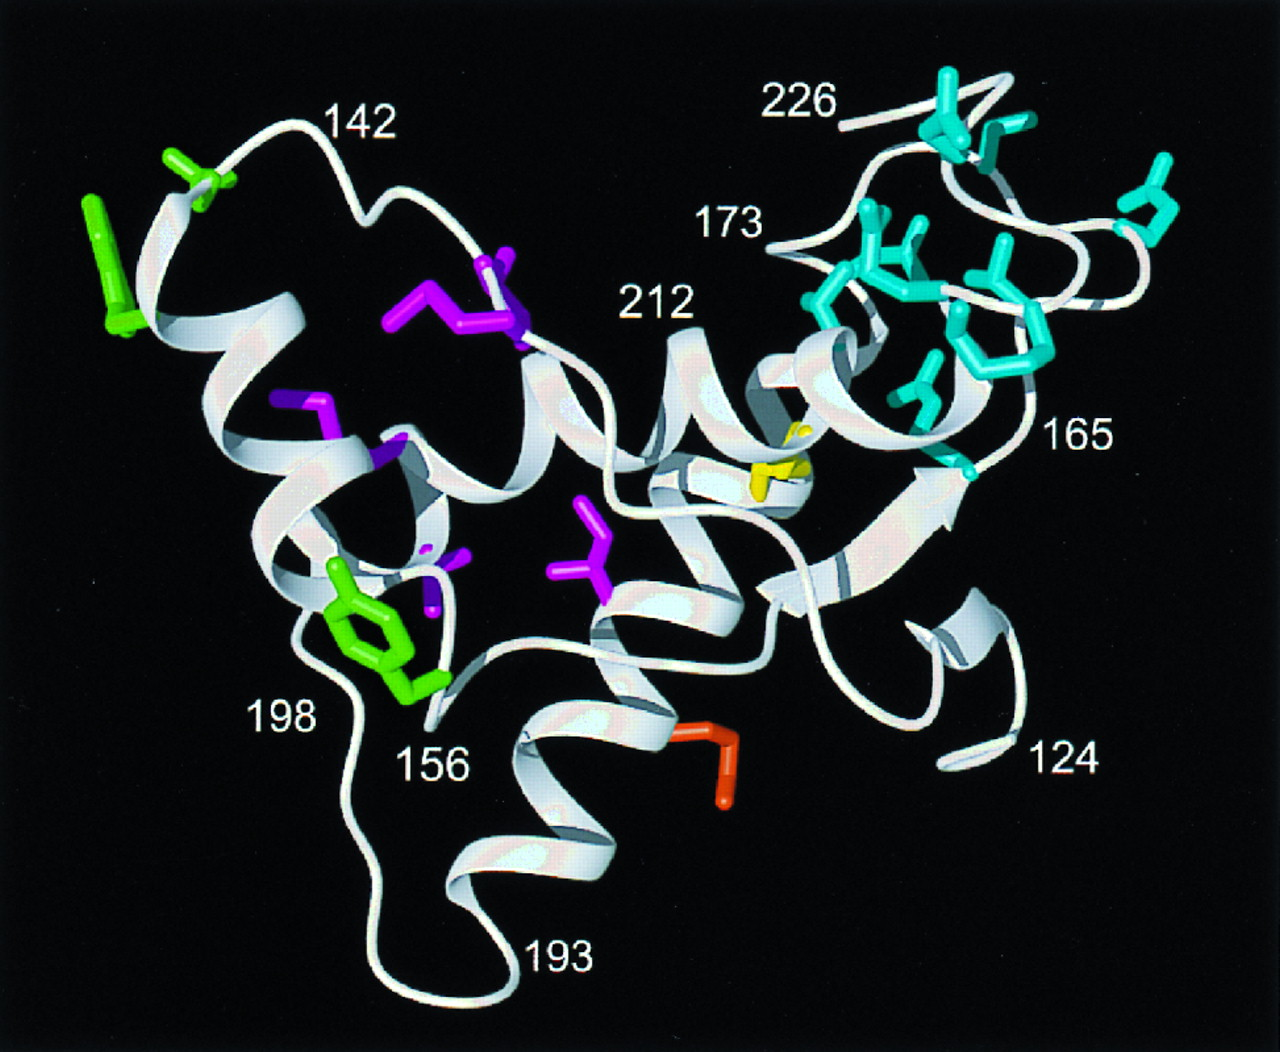
\includegraphics[width=\textwidth]{prion.jpg}
				\caption{NMR-derived structure of a prion  \url{http://www.pnas.org/content/94/14/7281.full}}
				\label{fig3}
			\end{minipage}					
		\end{figure}
	\end{frame}
	
	
	\begin{frame}{\thesection.\thesubsection. \insertsubsection}
		\begin{itemize}
			\item NMR relaxometry can be used to monitor molecular environment
		\end{itemize}

		\begin{figure}[ht]
					
						
			\begin{minipage}[t]{0.15\textwidth}
				\centering
				(a)
				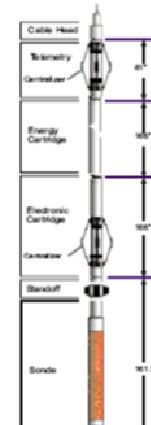
\includegraphics[width=\textwidth]{well_logging1.jpg}
			\end{minipage}
			\hspace{0.1cm}
			\begin{minipage}[t]{0.15\textwidth}
				\centering
				(b)
				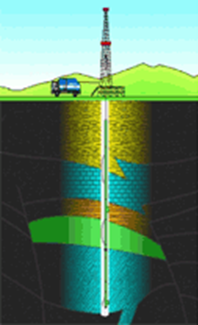
\includegraphics[width=\textwidth]{well_logging2.png}
				\label{fig7}
			\end{minipage}			
			\hspace{0.1cm}				
			\begin{minipage}[t]{0.15\textwidth}
				\centering
				(c)
				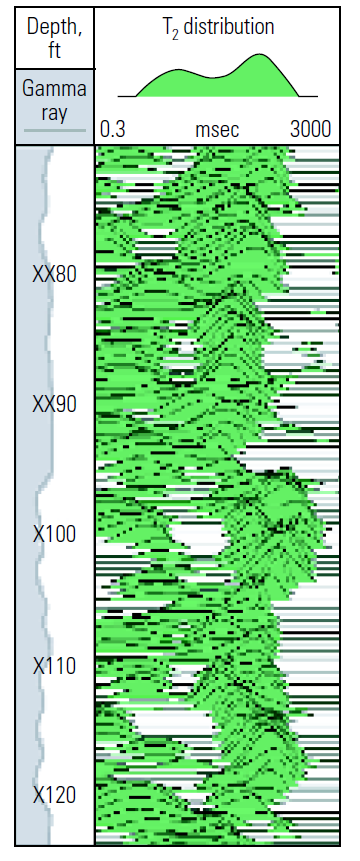
\includegraphics[width=\textwidth]{well_logging3.png}	
				\label{fig5}
			\end{minipage}		
			\hspace{0.1cm}
			\caption{ (a) NMR-logging probe, (b) Schematic positioning of the probe in a well, (c) T\textsubscript{2}-relaxation profile along the bore. Sources: 1) Allenet al. Oilfield review, Autumn 2000; 2) Coates, Xiao NMR Logging Principles and Applications, Hulliburton}		
		\end{figure}			
	\end{frame}
	
\begin{frame}{\thesection.\thesubsection. \insertsubsection}
	\begin{itemize}
		\item NMR forms the basis for magnetic resonance imaging (MRI)
	\end{itemize}
	
	\begin{figure}[ht]
			\centering
			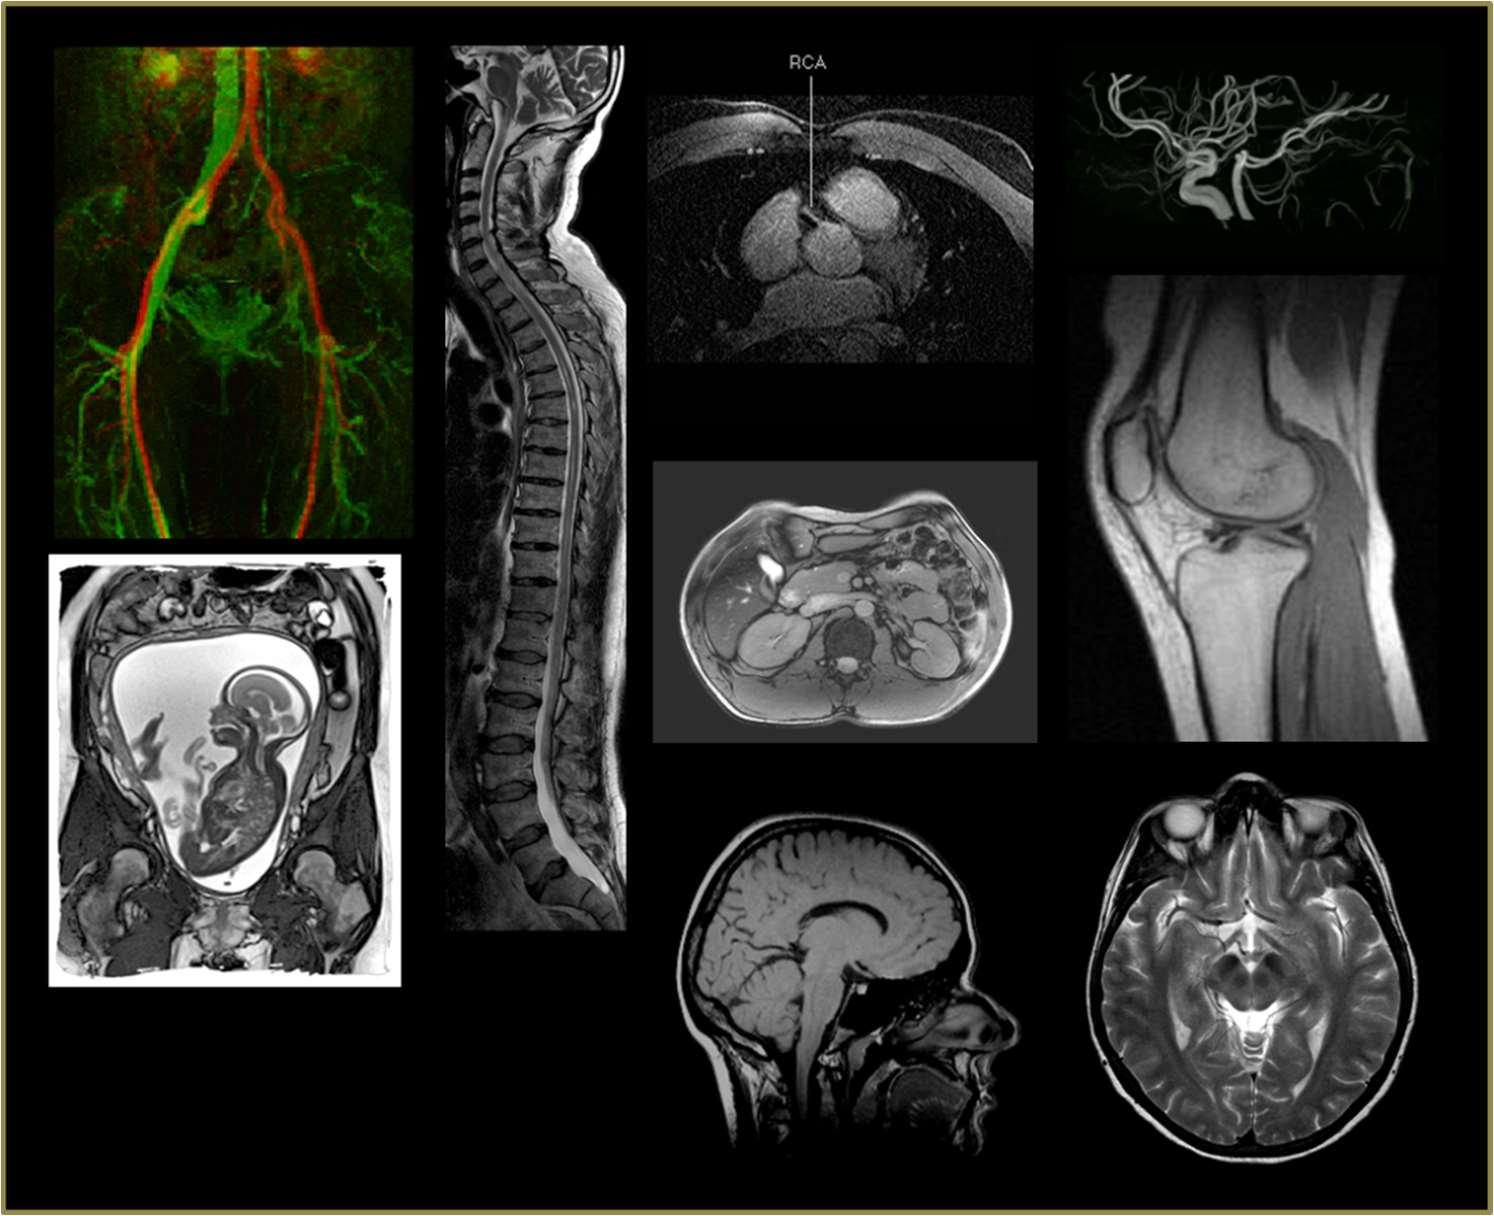
\includegraphics[width=0.7\textwidth]{mri.jpeg}
		\caption{  Example magnetic resonance images of blood vessel (in legs), fetus in utero, spine, heart, abdomen, head, blood vessels (in brain), knee, brain (courtesy of Prof. Richard Bowtell)}		
	\end{figure}			
\end{frame}


\subsection{Magnetic moments in magnetic field.}

\begin{frame}{\thesection.\thesubsection. \insertsubsection}
	
	\begin{itemize}[<+>]
		\item Consider charges moving in a limited volume. The position of a charge $\bm{e_n}$ will be given by a vector $\bm{r_n}$ and its velocity by $\bm{v_n}$. The overall magnetic moment of such a system is defined as:
			
			\begin{equation}
			\bm{M} = \frac{1}{2} \sum_{n} e_n\bm{r_n} \times \bm{v_n}
			\end{equation}
		\item 	If all the charges and masses are the same, then $\bm{M}$ can be rewritten as:	
			\begin{equation} \label{eq:1}
			\bm{M} = \frac{e}{2m} \sum_{n} m\bm{r_n} \times \bm{v_n} = \gamma \bm{L},
			\end{equation}
			where
			\begin{equation}
			\bm{L} = \sum_{n} \bm{p_n} \times \bm{r_n}
			\end{equation}
			is the mechanical angular momentum.
		\item 
			\alert{Gyromagnetic ratio}(or magnetogyric): 
			\begin{equation}
			\gamma = \dfrac{e}{2m}
			\end{equation}
			
	
	\end{itemize}
	


\end{frame}

\begin{frame}{\thesection.\thesubsection. \insertsubsection}
	\begin{itemize}[<+>]
		\item When a magnetic moment $\bm{M}$ is placed into an external uniform permanent magnetic field $\bm{B}$, its energy is given by:
			
			\begin{equation} \label{eq:classic_energy}
			E = -\bm{M} \cdot \bm{B}
			\end{equation} 
		\item  The torque acting on the system:
			\begin{equation}
			\frac{d\bm{L}}{dt} = \bm{M} \times \bm{B}
			\end{equation}
			  
		 \item  	Now using equation \ref{eq:1} we can obtain the equation describing the motion of vector $\bm{M}$:
			
			\begin{equation} \label{eq:precession_compact}
			\frac{d\bm{M}}{dt} = \gamma \bm{M} \times \bm{B}
			\end{equation}
			
	\end{itemize}
\end{frame}
\begin{frame}{\thesection.\thesubsection. \insertsubsection}
	\begin{itemize}[<+>]
		\item 
		    In a uniform magnetic field directed along $z$-axis $\bm{B} = (0, 0, B_0)$, the equation for individual components of $\bm{M}$ follow the equations:
		    
		    \begin{minipage}[b][4cm]{0.4\textwidth}
		    	\centering
		    	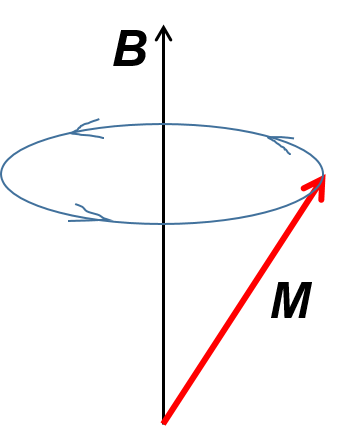
\includegraphics[width=0.7\textwidth]{precession.png}
		    \end{minipage}
		    \hspace{0.1cm}		    
		    \begin{minipage}[b][4cm]{0.4\textwidth}
		        \centering
		    	 \begin{equation} \label{precession}
		    	 \setlength{\jot}{5pt}
		    	 \begin{aligned}
		    	 \dfrac{dM_x}{dt} & =  \omega_L M_y \\
		    	 \dfrac{dM_y}{dt} & =  -\omega_L M_x \\
		    	 \dfrac{dM_z}{dt} & =  0,
		    	 \end{aligned}
		    	 \end{equation}
		    	 where $\omega_L = \gamma B_0$ - \alert{Larmor frequency}.
		    \end{minipage}
		    
		    
		\item
			A solution to this system of differential equations with initial values of $M_x(0), M_y(0), M_z(0)$ has the following form:
						
			\begin{equation} 
			\begin{array}{lcl}
			M_x(t) &=& M_x(0) \cos(\omega_L t) + M_y(0) \sin (\omega_L t) \\
			M_y(t) &=& -M_y(0) \sin(\omega_L t) + M_y(0) \cos (\omega_L t) \\
			M_z(t) &=& M_z(0) 
			\end{array}
			\end{equation}
		
		
	\end{itemize}
		
\end{frame}

\subsection{Orbital angular momentum operator}
\begin{frame}{\thesection.\thesubsection. \insertsubsection}
	
	\begin{itemize}[<+>]
		\item     In quantum mechanics physical quantities $A$ are represented by their operators $\hat{A}$. The mechanical angular momentum is replaced by its corresponding operator:
		\begin{equation}
		\bm{L} = \sum_{n} \bm{p_n} \times \bm{r_n}  \longleftrightarrow \bm{\hat{L}} = \dfrac{1}{\hbar} \sum_{n} \bm{\hat{r}_n} \times \bm{\hat{p}_n} =   -i \sum_{n} \bm{\hat{r}_n} \times \bm{\nabla_n}
		\end{equation}
		\item Angular momentum operator properties. Commutation:
		\begin{equation}\label{eq:Lz_commutation}
		  [\hat{L}_y,\hat{L}_z] = i\hat{L}_x, [\hat{L}_z,\hat{L}_x] = i\hat{L}_y, [\hat{L}_x,\hat{L}_y] = i\hat{L}_z
    	\end{equation}
		\item Angular momentum squared, and its commutation properties:
        \begin{align}
          &\hat{L}^2 = \hat{L}_x^2 + \hat{L}_y^2 + \hat{L}_z^2 \\
          &[\hat{L}^2, \hat{L}_x^2]=[\hat{L}^2, \hat{L}_y^2]=[\hat{L}^2, \hat{L}_z^2]= 0       
        \end{align}        
	\end{itemize}

\end{frame}

\begin{frame}{\thesection.\thesubsection. \insertsubsection}
	\begin{itemize}[<+>]
		\item Eigenfunctions of both $\hat{L}^2$ and $\hat{L}_z$ operators can be characterized by integer quantum numbers $l$  and $m$ respectively. These eigen functions will be denoted as $\vert lm \rangle$. Their eigenvalues are:
		\begin{align}
		\hat{L}_z \vert lm \rangle &= m \vert lm \rangle \\
		\hat{L}^2 \vert lm \rangle &= l(l+1) \vert lm \rangle
		\end{align}
		\item Another useful operator are raising and lowering operators:
		\begin{align}
		  &\hat{L}_{+} = \hat{L}_x + i\hat{L}_y, \hat{L}_{-} = \hat{L}_x - i\hat{L}_y\\
		  &\langle lm \vert \hat{L}_{+} \vert l (m-1) \rangle = \langle l(m-1) \vert \hat{L}_{-} \vert lm \rangle = \sqrt{(l+m)(l-m+1)} \label{eq:L+}
		\end{align}
	\end{itemize}
	
\end{frame}


\begin{frame}{\thesection.\thesubsection. \insertsubsection}
	\begin{itemize}[<+>]
		\item
			Classical magnetic moment will have its own quantum analogue, the operator of angular momentum:
			\begin{equation}\label{eq:orbital_angular_momentum}
			\bm{M} = \gamma \bm{L}  \longleftrightarrow \bm{\hat{\mu}} = \gamma \hbar \bm{\hat{L}}
			\end{equation} 
		\item Given the electron charge $e= 1.6 \cdot 10^{-19}$C, and mass $m = 9.1 \cdot 10^{-31}$kg   \alert{Bohr magneton}:
		\begin{equation}
			\beta_e = \gamma \hbar = \dfrac{e\hbar}{2m} \approx 9.27 \cdot 10^{-24}  \text{J$\cdot$T}^{-1}
		\end{equation}
		\item Similarly a \alert{nuclear magneton} could be calculated for a proton (\textsuperscript{1}H nucleus):
		\begin{equation}
		\beta = \gamma_N \hbar = \dfrac{e\hbar}{2m_p} \approx 5.05 \cdot 10^{-27}  \text{J$\cdot$T}^{-1}
		\end{equation}
		
	\end{itemize}

\end{frame}

\subsection{Spin angular momentum operator}
\begin{frame}{\thesection.\thesubsection. \insertsubsection}
	However, real nuclei and electrons have spins (intrinsic magnetic moment). Their z-axis projection $m$ takes integer and half-integer values: $m=\dfrac{1}{2}, 1, \dfrac{3}{2}, 2$ etc. Similar to the equation for the orbital angular momentum Eq.\ref{eq:orbital_angular_momentum}. For nuclei spins we get its magnetic moment as:
	\begin{equation}
		\bm{\hat{\mu}_N} = \gamma_N \hbar \bm{\hat{I}},
	\end{equation}
	where $ \bm{\hat{I}}$ stands for the nuclear spin operator. All the properties of angular momentum operators listed in Eqs.\ref{eq:Lz_commutation}-\ref*{eq:L+} will be true for $ \bm{\hat{I}}$.
\end{frame}

\begin{frame}{\thesection.\thesubsection. \insertsubsection}
	\begin{itemize}[<+>]
		\item 	Many nuclei in the periodic table are magnetic, i.e. have spin $I \neq 0$. Their magnetic moments could be measured in units of $\beta_N$:
		\begin{equation}
		\bm{\hat{\mu}_N} = \gamma_N \hbar \bm{\hat{I}} = g_N \beta_N \bm{\hat{I}},
		\end{equation}
		where $g_N$ - dimensionless g-factor.
		\item
% TABLE OF MAGNETIC PROPERTIES
\begin{table}[ht]
	\centering
	\begin{tabular}{  C{1.0cm}  C{2.0cm}  C{1.0cm}  C{2.cm}  C{3cm}}
		\hline\hline
		Nucleus & Natural abundance \% & Nuclear spin (I) & $g_N$, g-factor & $\gamma_N$, Gyromagnetic ratio ($10^7$ rad/T*s) \\
		\hline
		\textsuperscript{1}H & 99.98 & $\frac{1}{2}$ & 5.585 & 26.7519 \\
		\textsuperscript{2}H & 1.5*10\textsuperscript{-2} & 1 & 0.857 & 4.1066 \\
		\textsuperscript{13}C & 1.108 & $\frac{1}{2}$ & 1.405 & 6.7283 \\
		\textsuperscript{14}N & 99.635 & 1 & 0.403 & 1.9338 \\
		\textsuperscript{15}N & 0.365 &  $\frac{1}{2}$ & -0.567 & -2.712 \\
		\hline
	\end{tabular}
	%\caption{Magnetic properties of some common nuclei. More can be found at \url{http://www.bruker-nmr.de/guide/eNMR/chem/NMRnuclei.htm} }
	\label{tab:mag_properties}		
\end{table}
%%%%% END OF TABLE	
	\item
    Electron magnetic moments can be measured in units of Bohr magnetons: $\bm{\hat{\mu}_S} = -\gamma_e \hbar \bm{\hat{S}} = -g_e \beta_e \bm{\hat{S}}$, and for a free electron spin $g_e \approx 2.0023$.		
	\end{itemize}
\end{frame}


\subsection{Resonant absoption.}
%%%%%RESONANT ABSORBTION SECTION

\begin{frame}{\thesection.\thesubsection. \insertsubsection}
	\begin{itemize}[<+>]
		\item 
			Let's apply oscillating magnetic field to our system. A spin system Hamiltonian becomes time-dependent and for an oscillation along the $x$-axis we obtain:
			\begin{equation} \label{eq:oscillating_field}
			\begin{array}{lcl}
			\mathcal{H}(t) &=& -\bm{\hat{\mu}} \bm{(B_0+B(t))}=  \\
			&=& -\gamma \hbar \hat{I_z} (B_0 + B_1(t)) =\\
			&=&-\gamma \hbar \hat{I_z} B_0  -\gamma \hbar \hat{I_x} B_1 \cos(\omega t),
			\end{array}
			\end{equation}
			where $H_1$ and $\omega$ are the amplitude and the frequency of the oscillating magnetic field.
		\item
		 According to perturbation theory the transition probability between the initial state $\vert a \rangle$ and the final state $\vert b \rangle$ with a time dependent Hamiltonian $ \hat{V} (t) = 2 \hat{F} \cos (\omega t ) $ is (Fermi's golden rule):
		 \begin{equation} \label{eq:probability}
		 P_{ab} = \frac{2 \pi}{\hbar} \vert \langle a \vert \hat{F} \vert \rangle b \vert ^2 \delta(E_{ab}-\hbar \omega),
		 \end{equation}
		 where $E_{ab} = E_a - E_b$ is an energy difference between the energies of levels $a$ and $b$. 

		
	\end{itemize}
\end{frame}	

\begin{frame}{\thesection.\thesubsection. \insertsubsection}
	\begin{itemize}[]
		\item 
		For a two level system described before, the matrix element $\langle \alpha \vert \hat{I_x} \vert \beta \rangle = \frac{1}{2}$. The transition probability then becomes:
		\begin{equation}
		P_{\alpha \beta} = \frac{\pi}{2\hbar} (\gamma H_1)^2 \delta(E_{\alpha \beta}-\hbar \omega),
		\end{equation}
		\item
		    \textbf{The effect of resonant absorption (and emission) of electromagnetic irradiation at the frequency matching the energy difference in a nuclear system is called Nuclear Magnetic Resonance (NMR).} 		    
		    
		    
	\end{itemize}

\end{frame}	
\begin{frame}

	

\end{frame}
%%%%% END OF RESONANT ABSORPTION



\subsection{Spin in a magnetic field}
\begin{frame}{\thesection.\thesubsection. \insertsubsection}
		\begin{itemize}[<+>]
		\item Let's quantum mechanically describe the system of spins in the magnetic field. Eq. \ref{eq:classic_energy} can be rewritten in a form of Hamiltonian:
		\begin{equation}
			E = -\bm{M} \cdot \bm{B}  \longleftrightarrow \mathcal{H}= - \bm{\hat{\mu}_N} \cdot \bm{B} 
		\end{equation}
		\item when the magnetic field is directed along z-axis $\bm{B}= (0,0,B_0)$:
		\begin{equation}
		\mathcal{H}= - \bm{\hat{\mu}_N} \cdot \bm{B} = -\gamma_N \hbar B_0 \hat{I}_z
		\end{equation}
		\item For spin $I=\dfrac{1}{2}$ such Hamiltonian produces a two-level system. Its energy levels corresponding to eigenfunctions $\vert \alpha \rangle$ and $\vert \beta \rangle$:
		\begin{figure}
		    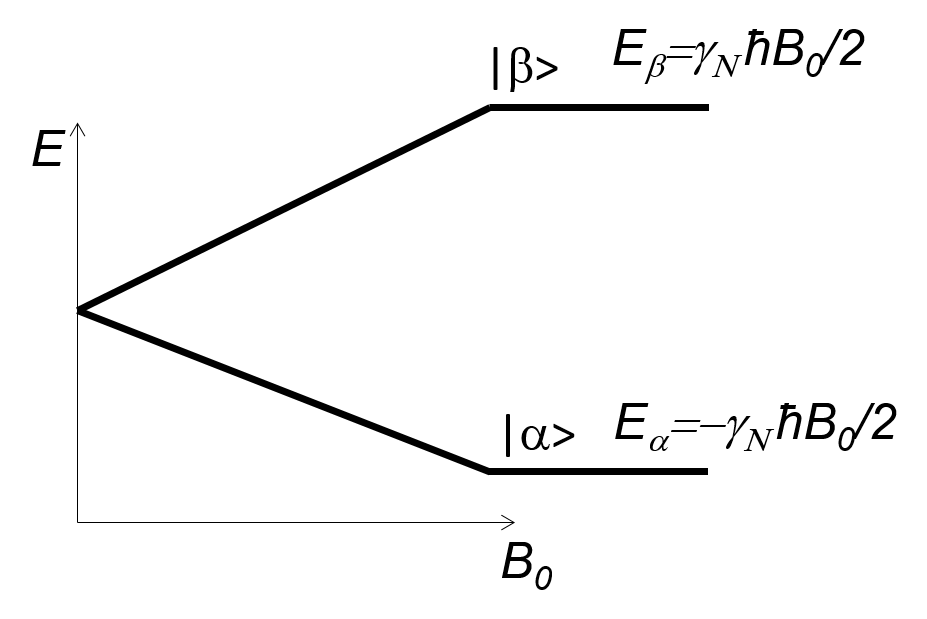
\includegraphics[width=0.5\textwidth]{two-level_system.png}
		\end{figure}
		
	\end{itemize}
\end{frame}

\begin{frame}{\thesection.\thesubsection. \insertsubsection}
	\begin{itemize}[<+>]
		\item The transition between the two states requires an energy quantum:
		\begin{equation}
			h \nu_L = \gamma \hbar B_0, \omega_L = \gamma B_0, \nu_L = \dfrac{\gamma B_0}{2 \pi}
		\end{equation}
		$\omega_L$ and $\nu_L$ is the Larmor frequency (anglular and cyclic respectively)
		\item
		
% TABLE OF MAGNETIC PROPERTIES
\begin{table}[ht]
	\centering
	\begin{tabular}{  C{1.0cm}  C{2.5cm}  C{1.0cm}  C{2.0cm}  C{2.0cm}}
		\hline\hline
		Nucleus & Natural abundance \% & Nuclear spin (I) & Larmor frequency at 11.744T, MHz & $\gamma_N$, Gyromagnetic ratio ($10^7$ rad/T*s) \\
		\hline
		\textsuperscript{1}H & 99.98 & $\frac{1}{2}$ & 500 & 26.7519 \\
		\textsuperscript{2}H & 1.5*10\textsuperscript{-2} & 1 & 76.753 & 4.1066 \\
		\textsuperscript{13}C & 1.108 & $\frac{1}{2}$ & 125.721 & 6.7283 \\
		\textsuperscript{14}N & 99.635 & 1 & 36.118 & 1.9338 \\
		\textsuperscript{15}N & 0.365 &  $\frac{1}{2}$ & 50.664 & -2.712 \\
		\hline
	\end{tabular}
\end{table}
%%%%% END OF TABLE
		
	\end{itemize}
\end{frame}

\subsection{Equilibrium magnetization}
\begin{frame}{\thesection.\thesubsection. \insertsubsection}
  NMR measurements are generally made on bulk samples which contain very large numbers of nuclear spins (e.g. 1 cm$^3$ contains $N \approx 6.7 \cdot 10^{22}$ \textsuperscript{1}H atoms)
  The measured signals therefore result from the collective effect of a large number of magnetic moments that can be described using a bulk magnetization.
  At thermal equilibrium, the numbers of nuclei in the $\vert \alpha \rangle$ state $N_{\alpha}$ and  $\vert \beta \rangle$ state $N_{beta}$ follow Boltzmann distribution:
  \begin{equation}
    \dfrac{N_{\alpha}}{N_{\beta}} = e^{-\dfrac{\gamma B_0}{kT}} \approx (1 - \dfrac{\gamma B_0}{kT}),
  \end{equation} 
  when $\gamma B_0 \ll kT$. Overall magnetization then can be calculated as:
  \begin{equation}
    M_z = N_{\alpha}(-\dfrac{1}{2}\gamma \hbar) + N_{\beta}(\dfrac{1}{2}\gamma \hbar) = N \dfrac{\gamma^2 \hbar^2 B_0}{4kT} 
  \end{equation}
\end{frame}




\begin{frame}

	These equations describe a precession of a vector $\bm{M}$ around the direction of the external magnetic field $\bm{B}$ with the frequency $\omega_0$ as shown schematically in Fig.\ref{fig:precession}A. Such motion is called  "Larmor precession" and $\omega_0 = \gamma B_0$ is called "Larmor frequency".
	
	Of course, this primitive classical picture serves only as an illustration to the actual behaviour of magnetic moments placed into a magnetic field. However, a more rigorous description using quantum mechanics for an ensemble of magnetic moments provides a similar answer. Larmor precession of an overall magnetic moment is a real effect, and as we will see later, it is essential for acquiring of magnetic resonance spectra.
	

	
	Now we'll briefly sketch the basic quantum mechanical description of a magnetic moment in a magnetic field.  The angular momentum operator $\bm{\hat{L}}$ (which could be an orbital or spin angular momentum) is proportional to the magnetic moment operator as:
	\begin{equation} \label{eq:3}
	\bm{\hat{\mu}} = \gamma \hbar \bm{\hat{L}},
	\end{equation}
	The Hamiltonian of a system can be written by analogy with expression \ref{eq:2} as:
	\begin{equation} \label{eq:2level}
	\hat{H} = -\bm{\hat{\mu}} \bm{B} = -\gamma \hbar \hat{I}_{z} B_0 = -\omega_0 \hat{I}_{z},
	\end{equation}
	
	The level diagram in Fig.\ref{fig:precession}B shows schematically the splitting of $\gamma \hbar B_0 $ between energy levels  as a function of the applied magnetic field for a system with only a spin-$\frac{1}{2}$ angular momentum. In this case, the eigenfunctions corresponding to the two energy levels are just the two projections of a spin onto the $z$-axis: $m_z=+\frac{1}{2}$ is $\vert \alpha \rangle$ and $m_z=-\frac{1}{2}$ is $\vert \beta \rangle$.
	
	
\end{frame}

\end{document}